\documentclass[tikz, border=2mm]{standalone}
\usepackage{amsmath}
\usepackage{tikz}
\usetikzlibrary{arrows.meta}

\begin{document}
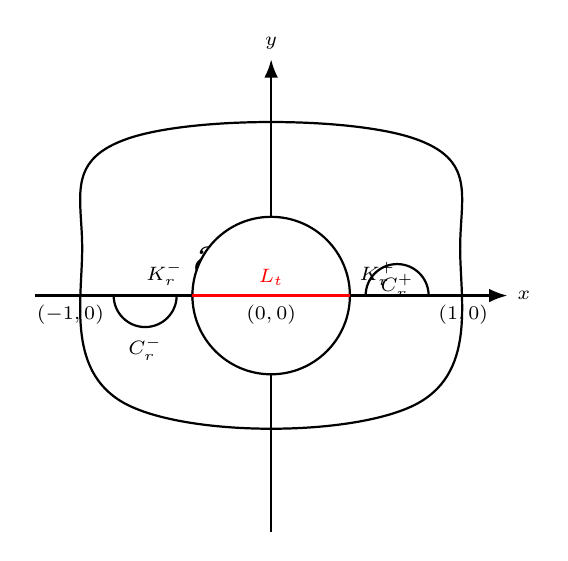
\begin{tikzpicture}[scale=2, every node/.style={font=\scriptsize}]

% Coordinate axes
\draw[-{Latex}, thick] (-1.5,0) -- (1.5,0) node[right] {$x$};
\draw[-{Latex}, thick] (0,-1.5) -- (0,1.5) node[above] {$y$};

% Outer boundary curve
\draw[thick] plot [smooth cycle, tension=0.7] coordinates {
    (-1.2,0.3) (-0.9,1) (0.9,1) (1.2,0.3) (0.9,-0.7) (-0.9,-0.7)
} node[above left, pos=0.2] {$\partial \Omega$};

% Small semicircles
\draw[thick] (-1,0) arc[start angle=180, end angle=360, radius=0.2]
    node[pos=0.5, below] {$C_{r}^{-}$};
\draw[thick] (1,0) arc[start angle=0, end angle=180, radius=0.2]
    node[pos=0.5, below] {$C_{r}^{+}$};

% Circles $K_{r}^{-}$ and $K_{r}^{+}$
\draw[thick] (0,0) ellipse (0.5 and 0.25);
\filldraw[white] (0,0) circle (0.5);
\draw[thick] (-0.5,0) arc[start angle=180, end angle=360, radius=0.5];
\draw[thick] (0.5,0) arc[start angle=0, end angle=180, radius=0.5];
\node at (-0.5,0) [above left] {$K_{r}^{-}$};
\node at (0.5,0) [above right] {$K_{r}^{+}$};

% Horizontal line segment $L_{t}$
\draw[red, thick] (-0.5,0) -- node[above, midway] {$L_{t}$} (0.5,0);

% Labels for points
\node at (-1,0) [below left] {$( -1 , 0 )$};
\node at (0,0) [below] {$( 0 , 0 )$};
\node at (1,0) [below right] {$( 1 , 0 )$};

\end{tikzpicture}
\end{document}